\documentclass[tikz,border=0pt]{standalone}
\usepackage{xcolor}
\usetikzlibrary{calc}
% Palette: Sam_Comm_final.png by eye, each course's own, and data/frogs.json.
\definecolor{ink}{HTML}{3B2340}
\definecolor{sky}{HTML}{EFC46A}
\definecolor{skyhi}{HTML}{F5DA92}
\definecolor{skylow}{HTML}{E9B060}
\definecolor{cloud}{HTML}{F2D58A}
\definecolor{paper}{HTML}{FBEFD0}
\definecolor{cream}{HTML}{FFF6E0}
\definecolor{white}{HTML}{FFFFFF}
\definecolor{wallA}{HTML}{E88A73}
\definecolor{wallB}{HTML}{EE9F7E}
\definecolor{wallC}{HTML}{E47A7E}
\definecolor{wallD}{HTML}{F0B07E}
\definecolor{wallE}{HTML}{D9765F}
\definecolor{wallF}{HTML}{E99A8A}
\definecolor{greenA}{HTML}{8DBB7E}
\definecolor{greenB}{HTML}{6FA77A}
\definecolor{greenC}{HTML}{A9C97F}
\definecolor{greenD}{HTML}{5E9C6A}
\definecolor{greenE}{HTML}{4A8060}
\definecolor{meadow}{HTML}{B5CF86}
\definecolor{meadowdark}{HTML}{9DBE74}
\definecolor{window}{HTML}{F6E7A0}
\definecolor{windark}{HTML}{8C5A64}
\definecolor{metal}{HTML}{8D9A93}
\definecolor{metaldark}{HTML}{5E6B66}
\definecolor{wood}{HTML}{B9835A}
\definecolor{wooddark}{HTML}{8C5A3C}
\definecolor{woodlight}{HTML}{D9A66F}
\definecolor{rope}{HTML}{E3C48A}
\definecolor{stone}{HTML}{E7C9A0}
\definecolor{stonedark}{HTML}{C9A47E}
\definecolor{road}{HTML}{8E7A86}
\definecolor{roadline}{HTML}{F6E7A0}
\definecolor{kerb}{HTML}{D8B48C}
\definecolor{red}{HTML}{E0483E}
\definecolor{redlight}{HTML}{F27A6A}
\definecolor{gold}{HTML}{FFB000}
\definecolor{goldlight}{HTML}{FFD54F}
\definecolor{bell}{HTML}{F2B53A}
\definecolor{teal}{HTML}{4FA3A0}
\definecolor{tealdark}{HTML}{3C8582}
\definecolor{magenta}{HTML}{FF2E88}
\definecolor{cyan}{HTML}{13CFE3}
\definecolor{violet}{HTML}{8A5BD6}
\definecolor{water}{HTML}{6FB3A8}
\definecolor{waterlight}{HTML}{9FD3C6}
\definecolor{waterdark}{HTML}{4F8E86}
\definecolor{pad}{HTML}{7DB86A}
\definecolor{paddark}{HTML}{5C9A52}
\definecolor{padlight}{HTML}{A6D38A}
\definecolor{reed}{HTML}{8DB26A}
\definecolor{cattail}{HTML}{8A5A3C}
\definecolor{moss}{HTML}{A8B88E}
\definecolor{cypress}{HTML}{5E8A5A}
\definecolor{cypressdark}{HTML}{4A7048}
\definecolor{lotus}{HTML}{F48FB1}
\definecolor{lotusdark}{HTML}{E06C98}
\definecolor{lotuslight}{HTML}{FAD0DF}
\definecolor{lotuscentre}{HTML}{FFD54F}
\definecolor{lotusseed}{HTML}{E0A82E}
\definecolor{flybody}{HTML}{2B2530}
\definecolor{flyeye}{HTML}{E0242E}
\definecolor{flywing}{HTML}{F4F8FA}
\definecolor{mushred}{HTML}{E23B2E}
\definecolor{mushspot}{HTML}{FFF5E0}
\definecolor{stem}{HTML}{F2E2C2}
\definecolor{blush}{HTML}{F48FB1}
\definecolor{pupil}{HTML}{1A1220}
\definecolor{spider}{HTML}{3B2340}
\definecolor{swampskyhi}{HTML}{E9E3A0}
\definecolor{swampsky}{HTML}{D9D184}
\definecolor{swampskylow}{HTML}{C9C478}
\definecolor{swampcloud}{HTML}{EEE9B4}
\definecolor{swampwater}{HTML}{4F8A7F}
\definecolor{swampwaterlight}{HTML}{7AAE9C}
\definecolor{swampwaterdark}{HTML}{3F7268}
\definecolor{log}{HTML}{9A6A48}
\definecolor{logend}{HTML}{D9A66F}
\definecolor{dunehi}{HTML}{F7DFA0}
\definecolor{dunesky}{HTML}{F2C47A}
\definecolor{duneskylow}{HTML}{EBA865}
\definecolor{sand}{HTML}{EBC27C}
\definecolor{sandlight}{HTML}{F4D69C}
\definecolor{sanddark}{HTML}{D9A35E}
\definecolor{sanddeep}{HTML}{C98C4E}
\definecolor{sun}{HTML}{FFE6A3}
\definecolor{cactus}{HTML}{6FA77A}
\definecolor{cactusdark}{HTML}{4F8A60}
\definecolor{palmtrunk}{HTML}{B98A5A}
\definecolor{rock}{HTML}{C98C6A}
\definecolor{awning}{HTML}{4FA3A0}
\definecolor{carA}{HTML}{4FA3A0}
\definecolor{carB}{HTML}{F2B53A}
\definecolor{carC}{HTML}{E47A7E}
\definecolor{carD}{HTML}{8DBB7E}
\definecolor{glass}{HTML}{BFE3E0}
\definecolor{duskhi}{HTML}{6B4A6E}
\definecolor{dusk}{HTML}{B9607A}
\definecolor{dusklow}{HTML}{E9906A}
\definecolor{duskcloud}{HTML}{8E6680}
\definecolor{smoke}{HTML}{9C8494}
\definecolor{smokedark}{HTML}{7E6878}
\definecolor{basalt}{HTML}{4A3A4A}
\definecolor{basaltdark}{HTML}{352838}
\definecolor{basalttop}{HTML}{6E5868}
\definecolor{rockface}{HTML}{5E4A5C}
\definecolor{lava}{HTML}{FF6A1A}
\definecolor{lavagold}{HTML}{FFB000}
\definecolor{lavadark}{HTML}{C9481A}
\definecolor{pool}{HTML}{5FB8B0}
\definecolor{poollight}{HTML}{9FE0D6}
\definecolor{fungskyhi}{HTML}{C9B6E4}
\definecolor{fungsky}{HTML}{DAC7EC}
\definecolor{fungskylow}{HTML}{EBD9F2}
\definecolor{fungcloud}{HTML}{F5ECF9}
\definecolor{fungmoss}{HTML}{8FB97E}
\definecolor{fungmossdark}{HTML}{6F9E72}
\definecolor{fungmosslight}{HTML}{B2D199}
\definecolor{farbark}{HTML}{A58BAE}
\definecolor{bumper}{HTML}{4A8FE7}
\definecolor{bumperlight}{HTML}{8FC4FF}
\definecolor{bumperspot}{HTML}{E6F2FF}
\definecolor{gill}{HTML}{EADBC0}
\definecolor{shelf}{HTML}{E8B07A}
\definecolor{shelfdark}{HTML}{C98C4E}
\definecolor{glowteal}{HTML}{4FD6C4}
\definecolor{glowtealhi}{HTML}{A8F2E6}
\definecolor{glowviolet}{HTML}{A77FE8}
\definecolor{glowviolethi}{HTML}{D9C4FF}
\definecolor{puff}{HTML}{F3EAD8}
\definecolor{puffdark}{HTML}{D9C9A8}
\definecolor{cliff}{HTML}{9C8AA8}
\definecolor{cliffdark}{HTML}{7E6C8C}
\definecolor{foam}{HTML}{F4FBFA}
\definecolor{bubble}{HTML}{D4F6F8}
\definecolor{bubbleteal}{HTML}{7FE0D8}
\definecolor{bubbleviolet}{HTML}{C9A8F0}
\definecolor{bubblepink}{HTML}{F7B8D8}
\definecolor{crown}{HTML}{FFC23A}
\definecolor{crowndark}{HTML}{E09A1A}
\definecolor{jewel}{HTML}{E0483E}
\definecolor{jewelb}{HTML}{4FA3A0}
\definecolor{limeskin}{HTML}{7BC043}
\definecolor{limebelly}{HTML}{F4E8B0}
\definecolor{limemark}{HTML}{3C7DC4}
\definecolor{limeeye}{HTML}{E23B2E}
\definecolor{limefeet}{HTML}{F2913D}
\definecolor{azureskin}{HTML}{2E6FD8}
\definecolor{azurebelly}{HTML}{1F4FA0}
\definecolor{azuremark}{HTML}{16163A}
\definecolor{azureeye}{HTML}{16163A}
\definecolor{azurefeet}{HTML}{1F4FA0}
\definecolor{bumbleskin}{HTML}{232028}
\definecolor{bumblebelly}{HTML}{2E2A33}
\definecolor{bumblemark}{HTML}{F6CF2E}
\definecolor{bumbleeye}{HTML}{16163A}
\definecolor{bumblefeet}{HTML}{232028}
\definecolor{tomatoskin}{HTML}{E2522F}
\definecolor{tomatobelly}{HTML}{F6D9B8}
\definecolor{tomatomark}{HTML}{B83A22}
\definecolor{tomatoeye}{HTML}{3A2A1E}
\definecolor{tomatofeet}{HTML}{C9442A}
\definecolor{bufoskin}{HTML}{9A7A4E}
\definecolor{bufobelly}{HTML}{E8D6A8}
\definecolor{bufomark}{HTML}{6B5233}
\definecolor{bufoeye}{HTML}{E8B83A}
\definecolor{bufofeet}{HTML}{8A6C44}
\definecolor{goldieskin}{HTML}{F59A1B}
\definecolor{goldiebelly}{HTML}{F8C25A}
\definecolor{goldiemark}{HTML}{D97C0E}
\definecolor{goldieeye}{HTML}{2A1A10}
\definecolor{goldiefeet}{HTML}{E8890F}
\definecolor{chompskin}{HTML}{A7C957}
\definecolor{chompbelly}{HTML}{F2E6B8}
\definecolor{chompmark}{HTML}{6A4A2E}
\definecolor{chompeye}{HTML}{C9A227}
\definecolor{chompfeet}{HTML}{8DAF45}
\definecolor{glassyskin}{HTML}{B9E3C6}
\definecolor{glassybelly}{HTML}{E4F4EA}
\definecolor{glassymark}{HTML}{F2E25C}
\definecolor{glassyeye}{HTML}{E9E0C8}
\definecolor{glassyfeet}{HTML}{9FD3B0}
\newcommand{\Ink}{1.15pt}
\tikzset{inked/.style={draw=ink, line width=\Ink, line join=round, line cap=round}}
\begin{document}
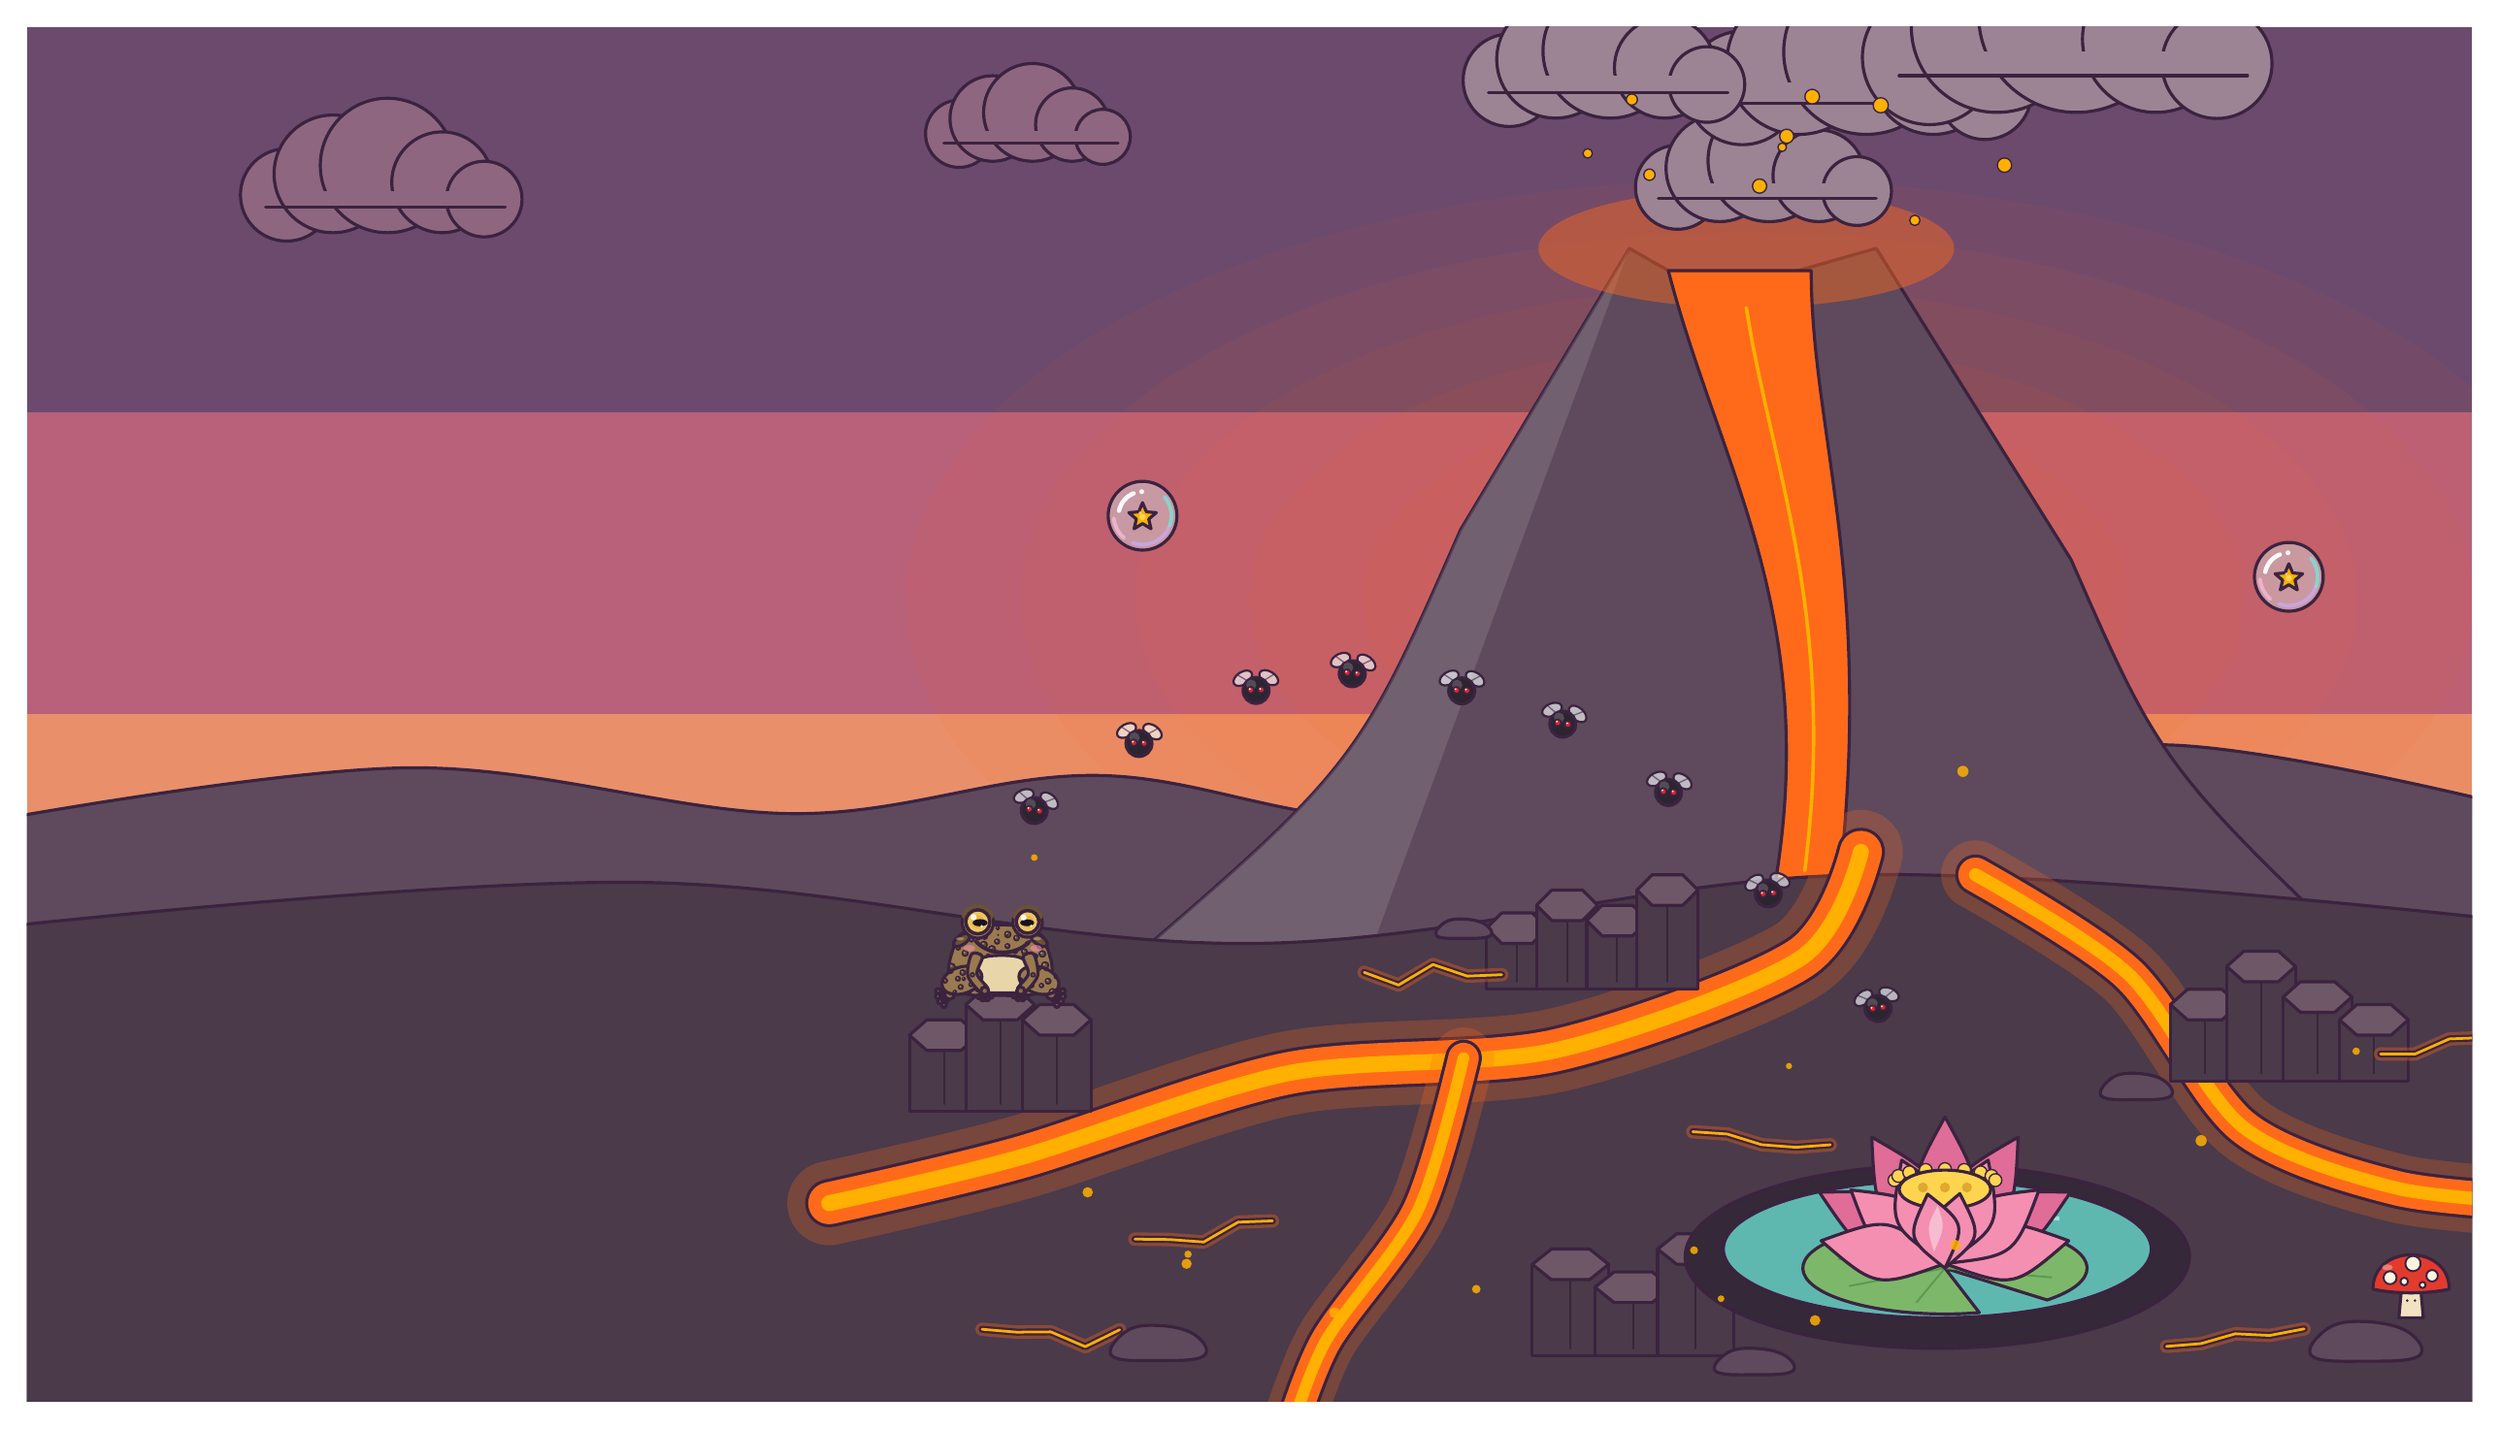
\begin{tikzpicture}
\clip (0,0) rectangle (32,18);
\fill[dusk] (0,0) rectangle (32,18);
\fill[duskhi] (0,12.96) rectangle (32,18);
\fill[dusklow] (0,0) rectangle (32,9);
\filldraw[inked,fill=duskcloud] (3.4,15.8) circle (0.605);
\filldraw[inked,fill=duskcloud] (4.005,16.075) circle (0.77);
\filldraw[inked,fill=duskcloud] (4.72,16.185) circle (0.88);
\filldraw[inked,fill=duskcloud] (5.435,15.965) circle (0.66);
\filldraw[inked,fill=duskcloud] (5.985,15.745) circle (0.495);
\fill[duskcloud] (3.4,15.635) rectangle (5.985,15.855);
\draw[ink, line width=1.15pt, line cap=round] (3.125,15.635) -- (6.26,15.635);
\filldraw[inked,fill=duskcloud] (12.2,16.6) circle (0.44);
\filldraw[inked,fill=duskcloud] (12.64,16.8) circle (0.56);
\filldraw[inked,fill=duskcloud] (13.16,16.88) circle (0.64);
\filldraw[inked,fill=duskcloud] (13.68,16.72) circle (0.48);
\filldraw[inked,fill=duskcloud] (14.08,16.56) circle (0.36);
\fill[duskcloud] (12.2,16.48) rectangle (14.08,16.64);
\draw[ink, line width=1.15pt, line cap=round] (12,16.48) -- (14.28,16.48);
\fill[lava, opacity=0.06] (22.5,10.5) ellipse (11 and 5.5);
\fill[lava, opacity=0.06] (22.5,10.5) ellipse (9.5 and 4.8);
\fill[lava, opacity=0.06] (22.5,10.5) ellipse (8 and 4.1);
\fill[lava, opacity=0.06] (22.5,10.5) ellipse (6.5 and 3.4);
\fill[lava, opacity=0.06] (22.5,10.5) ellipse (5 and 2.7);
\fill[lava, opacity=0.06] (22.5,10.5) ellipse (3.5 and 2);
\filldraw[inked,fill=rockface] plot[smooth, tension=0.6] coordinates {(-0.5,7.6) (5,8.3) (10,7.7) (14,8.2) (18,7.6) (24,8) (28,8.6) (32.5,7.8)} -- (32.5,-0.5) -- (-0.5,-0.5) -- cycle;
\filldraw[inked,fill=rockface] (14,5.4) .. controls (17.4,8.31) .. (18.76,11.414) -- (20.97,15.1) -- (21.82,14.615) -- (23.18,14.809) -- (24.2,15.1) -- (26.75,11.026) .. controls (27.94,8.31) .. (31,5.4) -- cycle;
\fill[white, opacity=0.12] (20.97,15.1) -- (18.76,11.414) .. controls (17.4,8.31) .. (14,5.4) -- (17.4,5.4) -- cycle;
\fill[lava, opacity=0.45] (22.5,15.1) ellipse (2.72 and 0.776);
\filldraw[inked,fill=lava] (21.48,14.809) .. controls (22.16,12.19) and (23.52,10.25) .. (22.84,6.564) -- (23.69,6.564) .. controls (24.2,10.735) and (23.35,12.675) .. (23.35,14.809) -- cycle;
\draw[lavagold, line width=1.3pt, line cap=round] (22.5,14.324) .. controls (22.84,12.19) and (23.69,10.25) .. (23.265,6.952);
\filldraw[inked,fill=smoke] (21.6,15.9) circle (0.55);
\filldraw[inked,fill=smoke] (22.15,16.15) circle (0.7);
\filldraw[inked,fill=smoke] (22.8,16.25) circle (0.8);
\filldraw[inked,fill=smoke] (23.45,16.05) circle (0.6);
\filldraw[inked,fill=smoke] (23.95,15.85) circle (0.45);
\fill[smoke] (21.6,15.75) rectangle (23.95,15.95);
\draw[ink, line width=1.15pt, line cap=round] (21.35,15.75) -- (24.2,15.75);
\filldraw[inked,fill=smoke] (22.45,17.2) circle (0.743);
\filldraw[inked,fill=smoke] (23.192,17.537) circle (0.945);
\filldraw[inked,fill=smoke] (24.07,17.672) circle (1.08);
\filldraw[inked,fill=smoke] (24.948,17.402) circle (0.81);
\filldraw[inked,fill=smoke] (25.623,17.133) circle (0.608);
\fill[smoke] (22.45,16.997) rectangle (25.623,17.267);
\draw[ink, line width=1.15pt, line cap=round] (22.113,16.997) -- (25.96,16.997);
\filldraw[inked,fill=smoke] (24.9,17.6) circle (0.88);
\filldraw[inked,fill=smoke] (25.78,18) circle (1.12);
\filldraw[inked,fill=smoke] (26.82,18.16) circle (1.28);
\filldraw[inked,fill=smoke] (27.86,17.84) circle (0.96);
\filldraw[inked,fill=smoke] (28.66,17.52) circle (0.72);
\fill[smoke] (24.9,17.36) rectangle (28.66,17.68);
\draw[ink, line width=1.15pt, line cap=round] (24.5,17.36) -- (29.06,17.36);
\filldraw[inked,fill=smoke] (19.4,17.3) circle (0.605);
\filldraw[inked,fill=smoke] (20.005,17.575) circle (0.77);
\filldraw[inked,fill=smoke] (20.72,17.685) circle (0.88);
\filldraw[inked,fill=smoke] (21.435,17.465) circle (0.66);
\filldraw[inked,fill=smoke] (21.985,17.245) circle (0.495);
\fill[smoke] (19.4,17.135) rectangle (21.985,17.355);
\draw[ink, line width=1.15pt, line cap=round] (19.125,17.135) -- (22.26,17.135);
\filldraw[inked,fill=lavagold,line width=0.5pt] (20.425,16.343) circle (0.062);
\filldraw[inked,fill=lavagold,line width=0.5pt] (22.674,15.915) circle (0.093);
\filldraw[inked,fill=lavagold,line width=0.5pt] (23.363,17.086) circle (0.096);
\filldraw[inked,fill=lavagold,line width=0.5pt] (22.97,16.424) circle (0.056);
\filldraw[inked,fill=lavagold,line width=0.5pt] (24.706,15.467) circle (0.068);
\filldraw[inked,fill=lavagold,line width=0.5pt] (21.003,17.048) circle (0.073);
\filldraw[inked,fill=lavagold,line width=0.5pt] (23.029,16.568) circle (0.092);
\filldraw[inked,fill=lavagold,line width=0.5pt] (25.879,16.189) circle (0.094);
\filldraw[inked,fill=lavagold,line width=0.5pt] (24.26,16.973) circle (0.099);
\filldraw[inked,fill=lavagold,line width=0.5pt] (21.233,16.064) circle (0.074);
\filldraw[inked,fill=basalt] plot[smooth, tension=0.6] coordinates {(-0.5,6.2) (8,6.8) (16,6) (24,6.9) (32.5,6.3)} -- (32.5,-0.5) -- (-0.5,-0.5) -- cycle;
\draw[lava, opacity=0.25, line width=31.298pt, line cap=round, line join=round] plot[smooth] coordinates {(24,7.2) (23.2,5.8) (20,4.6) (16.5,4.3) (13,3.2) (10.5,2.6)};
\draw[ink, line width=17.949pt, line cap=round, line join=round] plot[smooth] coordinates {(24,7.2) (23.2,5.8) (20,4.6) (16.5,4.3) (13,3.2) (10.5,2.6)};
\draw[lava, line width=15.649pt, line cap=round, line join=round] plot[smooth] coordinates {(24,7.2) (23.2,5.8) (20,4.6) (16.5,4.3) (13,3.2) (10.5,2.6)};
\draw[lavagold, line width=5.947pt, line cap=round, line join=round] plot[smooth] coordinates {(24,7.2) (23.2,5.8) (20,4.6) (16.5,4.3) (13,3.2) (10.5,2.6)};
\draw[lava, opacity=0.25, line width=25.608pt, line cap=round, line join=round] plot[smooth] coordinates {(25.5,6.9) (27.5,5.6) (29,3.6) (31,2.8) (33,2.6)};
\draw[ink, line width=15.104pt, line cap=round, line join=round] plot[smooth] coordinates {(25.5,6.9) (27.5,5.6) (29,3.6) (31,2.8) (33,2.6)};
\draw[lava, line width=12.804pt, line cap=round, line join=round] plot[smooth] coordinates {(25.5,6.9) (27.5,5.6) (29,3.6) (31,2.8) (33,2.6)};
\draw[lavagold, line width=4.865pt, line cap=round, line join=round] plot[smooth] coordinates {(25.5,6.9) (27.5,5.6) (29,3.6) (31,2.8) (33,2.6)};
\draw[lava, opacity=0.25, line width=22.762pt, line cap=round, line join=round] plot[smooth] coordinates {(18.8,4.5) (18.2,2.5) (17,0.8) (16.5,-0.5)};
\draw[ink, line width=13.681pt, line cap=round, line join=round] plot[smooth] coordinates {(18.8,4.5) (18.2,2.5) (17,0.8) (16.5,-0.5)};
\draw[lava, line width=11.381pt, line cap=round, line join=round] plot[smooth] coordinates {(18.8,4.5) (18.2,2.5) (17,0.8) (16.5,-0.5)};
\draw[lavagold, line width=4.325pt, line cap=round, line join=round] plot[smooth] coordinates {(18.8,4.5) (18.2,2.5) (17,0.8) (16.5,-0.5)};
\filldraw[inked,fill=basalt] (11.55,3.8) -- (12.45,3.8) -- (12.45,4.8) -- (11.55,4.8) -- cycle;
\draw[basaltdark, line width=0.7pt, line cap=round] (12,3.9) -- (12,4.6);
\filldraw[inked,fill=basalttop] (11.55,4.8) -- (11.775,5) -- (12.225,5) -- (12.45,4.8) -- (12.225,4.6) -- (11.775,4.6) -- cycle;
\filldraw[inked,fill=basalt] (12.288,3.8) -- (13.188,3.8) -- (13.188,5.2) -- (12.288,5.2) -- cycle;
\draw[basaltdark, line width=0.7pt, line cap=round] (12.738,3.9) -- (12.738,5);
\filldraw[inked,fill=basalttop] (12.288,5.2) -- (12.513,5.4) -- (12.963,5.4) -- (13.188,5.2) -- (12.963,5) -- (12.513,5) -- cycle;
\filldraw[inked,fill=basalt] (13.026,3.8) -- (13.926,3.8) -- (13.926,5) -- (13.026,5) -- cycle;
\draw[basaltdark, line width=0.7pt, line cap=round] (13.476,3.9) -- (13.476,4.8);
\filldraw[inked,fill=basalttop] (13.026,5) -- (13.251,5.2) -- (13.701,5.2) -- (13.926,5) -- (13.701,4.8) -- (13.251,4.8) -- cycle;
\begin{scope}[shift={(12.74,5.32)}, rotate=0, xscale=0.3, yscale=0.3]
\filldraw[inked,fill=bufofeet] (-2.218,0.05) .. controls (-2.243,-0.231) .. (-2.462,-0.409) .. controls (-2.437,-0.128) .. (-2.218,0.05) -- cycle;
\filldraw[inked,fill=bufofeet] (-2.462,-0.409) circle (0.11);
\filldraw[inked,fill=bufofeet] (-2.218,0.05) .. controls (-2.363,-0.192) .. (-2.638,-0.256) .. controls (-2.493,-0.014) .. (-2.218,0.05) -- cycle;
\filldraw[inked,fill=bufofeet] (-2.638,-0.256) circle (0.11);
\filldraw[inked,fill=bufofeet] (-2.218,0.05) .. controls (-2.455,-0.103) .. (-2.73,-0.04) .. controls (-2.493,0.113) .. (-2.218,0.05) -- cycle;
\filldraw[inked,fill=bufofeet] (-2.73,-0.04) circle (0.11);
\filldraw[inked,fill=bufofeet] (-2.218,0.05) .. controls (-2.498,0.016) .. (-2.717,0.193) .. controls (-2.437,0.227) .. (-2.218,0.05) -- cycle;
\filldraw[inked,fill=bufofeet] (-2.717,0.193) circle (0.11);
\filldraw[inked,fill=bufofeet] (-2.218,0.05) circle (0.22);
\filldraw[inked,fill=bufofeet] (2.218,0.05) .. controls (2.437,-0.128) .. (2.462,-0.409) .. controls (2.243,-0.231) .. (2.218,0.05) -- cycle;
\filldraw[inked,fill=bufofeet] (2.462,-0.409) circle (0.11);
\filldraw[inked,fill=bufofeet] (2.218,0.05) .. controls (2.493,-0.014) .. (2.638,-0.256) .. controls (2.363,-0.192) .. (2.218,0.05) -- cycle;
\filldraw[inked,fill=bufofeet] (2.638,-0.256) circle (0.11);
\filldraw[inked,fill=bufofeet] (2.218,0.05) .. controls (2.493,0.113) .. (2.73,-0.04) .. controls (2.455,-0.103) .. (2.218,0.05) -- cycle;
\filldraw[inked,fill=bufofeet] (2.73,-0.04) circle (0.11);
\filldraw[inked,fill=bufofeet] (2.218,0.05) .. controls (2.437,0.227) .. (2.717,0.193) .. controls (2.498,0.016) .. (2.218,0.05) -- cycle;
\filldraw[inked,fill=bufofeet] (2.717,0.193) circle (0.11);
\filldraw[inked,fill=bufofeet] (2.218,0.05) circle (0.22);
\fill[bufoskin] plot[smooth cycle, tension=0.7] coordinates {(0,0) (1.624,0.097) (2.218,0.776) (2.106,1.891) (1.568,2.764) (0,3.085) (-1.568,2.764) (-2.106,1.891) (-2.218,0.776) (-1.624,0.097)};
\begin{scope}\clip plot[smooth cycle, tension=0.7] coordinates {(0,0) (1.624,0.097) (2.218,0.776) (2.106,1.891) (1.568,2.764) (0,3.085) (-1.568,2.764) (-2.106,1.891) (-2.218,0.776) (-1.624,0.097)};
\filldraw[inked,fill=bufomark,line width=0.6pt] (1.535,1.714) circle (0.085);
\fill[bufobelly, opacity=0.55] (1.509,1.739) circle (0.03);
\filldraw[inked,fill=bufomark,line width=0.6pt] (-0.994,0.921) circle (0.127);
\fill[bufobelly, opacity=0.55] (-1.032,0.959) circle (0.044);
\filldraw[inked,fill=bufomark,line width=0.6pt] (1.131,1.493) circle (0.14);
\fill[bufobelly, opacity=0.55] (1.089,1.535) circle (0.049);
\filldraw[inked,fill=bufomark,line width=0.6pt] (-2.217,0.587) circle (0.081);
\fill[bufobelly, opacity=0.55] (-2.241,0.611) circle (0.028);
\filldraw[inked,fill=bufomark,line width=0.6pt] (1.731,2.162) circle (0.127);
\fill[bufobelly, opacity=0.55] (1.693,2.2) circle (0.044);
\filldraw[inked,fill=bufomark,line width=0.6pt] (-1.845,2.082) circle (0.091);
\fill[bufobelly, opacity=0.55] (-1.873,2.11) circle (0.032);
\filldraw[inked,fill=bufomark,line width=0.6pt] (-0.685,2.576) circle (0.119);
\fill[bufobelly, opacity=0.55] (-0.721,2.612) circle (0.042);
\filldraw[inked,fill=bufomark,line width=0.6pt] (0.319,2.66) circle (0.131);
\fill[bufobelly, opacity=0.55] (0.28,2.699) circle (0.046);
\filldraw[inked,fill=bufomark,line width=0.6pt] (-1.218,0.426) circle (0.073);
\fill[bufobelly, opacity=0.55] (-1.24,0.448) circle (0.025);
\filldraw[inked,fill=bufomark,line width=0.6pt] (-0.37,1.505) circle (0.077);
\fill[bufobelly, opacity=0.55] (-0.393,1.528) circle (0.027);
\filldraw[inked,fill=bufomark,line width=0.6pt] (-1.683,0.966) circle (0.14);
\fill[bufobelly, opacity=0.55] (-1.725,1.008) circle (0.049);
\filldraw[inked,fill=bufomark,line width=0.6pt] (-1.018,3.094) circle (0.111);
\fill[bufobelly, opacity=0.55] (-1.051,3.127) circle (0.039);
\filldraw[inked,fill=bufomark,line width=0.6pt] (2.21,1.72) circle (0.087);
\fill[bufobelly, opacity=0.55] (2.184,1.746) circle (0.03);
\filldraw[inked,fill=bufomark,line width=0.6pt] (-0.702,0.494) circle (0.098);
\fill[bufobelly, opacity=0.55] (-0.731,0.524) circle (0.034);
\filldraw[inked,fill=bufomark,line width=0.6pt] (0.647,1.922) circle (0.088);
\fill[bufobelly, opacity=0.55] (0.621,1.949) circle (0.031);
\filldraw[inked,fill=bufomark,line width=0.6pt] (1.949,1.309) circle (0.149);
\fill[bufobelly, opacity=0.55] (1.904,1.354) circle (0.052);
\filldraw[inked,fill=bufomark,line width=0.6pt] (-0.02,1.021) circle (0.07);
\fill[bufobelly, opacity=0.55] (-0.041,1.042) circle (0.025);
\filldraw[inked,fill=bufomark,line width=0.6pt] (1.046,1.908) circle (0.116);
\fill[bufobelly, opacity=0.55] (1.011,1.943) circle (0.041);
\filldraw[inked,fill=bufomark,line width=0.6pt] (-0.49,2.83) circle (0.102);
\fill[bufobelly, opacity=0.55] (-0.521,2.86) circle (0.036);
\filldraw[inked,fill=bufomark,line width=0.6pt] (-0.37,2.018) circle (0.145);
\fill[bufobelly, opacity=0.55] (-0.413,2.062) circle (0.051);
\filldraw[inked,fill=bufomark,line width=0.6pt] (0.31,2.153) circle (0.097);
\fill[bufobelly, opacity=0.55] (0.281,2.182) circle (0.034);
\filldraw[inked,fill=bufomark,line width=0.6pt] (0.703,2.504) circle (0.111);
\fill[bufobelly, opacity=0.55] (0.669,2.537) circle (0.039);
\filldraw[inked,fill=bufomark,line width=0.6pt] (-0.346,0.822) circle (0.12);
\fill[bufobelly, opacity=0.55] (-0.382,0.858) circle (0.042);
\filldraw[inked,fill=bufomark,line width=0.6pt] (-0.723,2.215) circle (0.139);
\fill[bufobelly, opacity=0.55] (-0.765,2.256) circle (0.049);
\filldraw[inked,fill=bufomark,line width=0.6pt] (1.015,0.561) circle (0.14);
\fill[bufobelly, opacity=0.55] (0.973,0.603) circle (0.049);
\filldraw[inked,fill=bufomark,line width=0.6pt] (-0.976,2.516) circle (0.091);
\fill[bufobelly, opacity=0.55] (-1.004,2.543) circle (0.032);
\filldraw[inked,fill=bufomark,line width=0.6pt] (-1.207,2.902) circle (0.071);
\fill[bufobelly, opacity=0.55] (-1.228,2.923) circle (0.025);
\filldraw[inked,fill=bufomark,line width=0.6pt] (2.096,2.118) circle (0.118);
\fill[bufobelly, opacity=0.55] (2.06,2.154) circle (0.041);
\filldraw[inked,fill=bufomark,line width=0.6pt] (-0.819,1.22) circle (0.073);
\fill[bufobelly, opacity=0.55] (-0.841,1.241) circle (0.026);
\filldraw[inked,fill=bufomark,line width=0.6pt] (2.235,0.506) circle (0.076);
\fill[bufobelly, opacity=0.55] (2.213,0.529) circle (0.027);
\filldraw[inked,fill=bufomark,line width=0.6pt] (1.832,1.81) circle (0.133);
\fill[bufobelly, opacity=0.55] (1.792,1.85) circle (0.047);
\filldraw[inked,fill=bufomark,line width=0.6pt] (-1.251,2.433) circle (0.09);
\fill[bufobelly, opacity=0.55] (-1.278,2.46) circle (0.031);
\filldraw[inked,fill=bufomark,line width=0.6pt] (1.694,0.807) circle (0.114);
\fill[bufobelly, opacity=0.55] (1.66,0.842) circle (0.04);
\filldraw[inked,fill=bufomark,line width=0.6pt] (-0.145,2.351) circle (0.103);
\fill[bufobelly, opacity=0.55] (-0.176,2.381) circle (0.036);
\filldraw[inked,fill=bufomark,line width=0.6pt] (0.669,1.338) circle (0.094);
\fill[bufobelly, opacity=0.55] (0.641,1.366) circle (0.033);
\filldraw[inked,fill=bufomark,line width=0.6pt] (-1.539,1.842) circle (0.124);
\fill[bufobelly, opacity=0.55] (-1.576,1.879) circle (0.043);
\filldraw[inked,fill=bufomark,line width=0.6pt] (0.813,1.615) circle (0.082);
\fill[bufobelly, opacity=0.55] (0.788,1.64) circle (0.029);
\filldraw[inked,fill=bufomark,line width=0.6pt] (-1.38,0.176) circle (0.105);
\fill[bufobelly, opacity=0.55] (-1.412,0.207) circle (0.037);
\filldraw[inked,fill=bufomark,line width=0.6pt] (1.656,0.204) circle (0.142);
\fill[bufobelly, opacity=0.55] (1.613,0.246) circle (0.05);
\filldraw[inked,fill=bufomark,line width=0.6pt] (1.455,2.852) circle (0.082);
\fill[bufobelly, opacity=0.55] (1.43,2.876) circle (0.029);
\filldraw[inked,fill=bufomark,line width=0.6pt] (-0.929,1.662) circle (0.139);
\fill[bufobelly, opacity=0.55] (-0.97,1.703) circle (0.048);
\filldraw[inked,fill=bufomark,line width=0.6pt] (-2.065,2.617) circle (0.099);
\fill[bufobelly, opacity=0.55] (-2.094,2.646) circle (0.035);
\filldraw[inked,fill=bufomark,line width=0.6pt] (1.079,2.618) circle (0.081);
\fill[bufobelly, opacity=0.55] (1.055,2.643) circle (0.028);
\filldraw[inked,fill=bufomark,line width=0.6pt] (-0.114,2.946) circle (0.074);
\fill[bufobelly, opacity=0.55] (-0.136,2.968) circle (0.026);
\filldraw[inked,fill=bufomark,line width=0.6pt] (0.011,0.608) circle (0.14);
\fill[bufobelly, opacity=0.55] (-0.031,0.65) circle (0.049);
\filldraw[inked,fill=bufomark,line width=0.6pt] (2.239,2.971) circle (0.146);
\fill[bufobelly, opacity=0.55] (2.196,3.014) circle (0.051);
\filldraw[inked,fill=bufomark,line width=0.6pt] (1.173,2.274) circle (0.077);
\fill[bufobelly, opacity=0.55] (1.15,2.297) circle (0.027);
\filldraw[inked,fill=bufomark,line width=0.6pt] (-2.124,1.251) circle (0.141);
\fill[bufobelly, opacity=0.55] (-2.166,1.293) circle (0.049);
\filldraw[inked,fill=bufomark,line width=0.6pt] (0.2,0.278) circle (0.111);
\fill[bufobelly, opacity=0.55] (0.167,0.311) circle (0.039);
\filldraw[inked,fill=bufomark,line width=0.6pt] (-0.53,1.715) circle (0.087);
\fill[bufobelly, opacity=0.55] (-0.556,1.741) circle (0.03);
\filldraw[inked,fill=bufomark,line width=0.6pt] (2.028,0.634) circle (0.079);
\fill[bufobelly, opacity=0.55] (2.005,0.657) circle (0.027);
\filldraw[inked,fill=bufomark,line width=0.6pt] (1.996,2.536) circle (0.101);
\fill[bufobelly, opacity=0.55] (1.966,2.566) circle (0.035);
\filldraw[inked,fill=bufomark,line width=0.6pt] (-2.112,2.926) circle (0.099);
\fill[bufobelly, opacity=0.55] (-2.142,2.956) circle (0.035);
\end{scope}
\draw[inked] plot[smooth cycle, tension=0.7] coordinates {(0,0) (1.624,0.097) (2.218,0.776) (2.106,1.891) (1.568,2.764) (0,3.085) (-1.568,2.764) (-2.106,1.891) (-2.218,0.776) (-1.624,0.097)};
\filldraw[inked,fill=bufomark,rotate around={35:(-1.68,2.425)}] (-1.68,2.425) ellipse (0.42 and 0.2);
\fill[bufobelly, opacity=0.4] (-1.76,2.473) ellipse (0.18 and 0.07);
\filldraw[inked,fill=bufomark,rotate around={-35:(1.68,2.425)}] (1.68,2.425) ellipse (0.42 and 0.2);
\fill[bufobelly, opacity=0.4] (1.6,2.473) ellipse (0.18 and 0.07);
\fill[bufobelly] plot[smooth cycle, tension=0.7] coordinates {(0.05,0.116) (1.114,0.213) (1.338,0.873) (1.058,1.552) (0.05,1.746) (-0.958,1.552) (-1.238,0.873) (-1.014,0.213)};
\draw[inked] plot[smooth cycle, tension=0.7] coordinates {(0.05,0.116) (1.114,0.213) (1.338,0.873) (1.058,1.552) (0.05,1.746) (-0.958,1.552) (-1.238,0.873) (-1.014,0.213)};
\fill[bufoskin] [rotate around={18:(-1.68,0.66)}] (-1.68,0.66) ellipse (0.896 and 0.58);
\begin{scope}\clip [rotate around={18:(-1.68,0.66)}] (-1.68,0.66) ellipse (0.896 and 0.58);
\filldraw[inked,fill=bufomark,line width=0.6pt] (-1.851,0.729) circle (0.095);
\fill[bufobelly, opacity=0.55] (-1.879,0.757) circle (0.033);
\filldraw[inked,fill=bufomark,line width=0.6pt] (-0.828,0.444) circle (0.148);
\fill[bufobelly, opacity=0.55] (-0.873,0.488) circle (0.052);
\filldraw[inked,fill=bufomark,line width=0.6pt] (-1.086,0.85) circle (0.118);
\fill[bufobelly, opacity=0.55] (-1.121,0.886) circle (0.041);
\filldraw[inked,fill=bufomark,line width=0.6pt] (-1.73,0.368) circle (0.098);
\fill[bufobelly, opacity=0.55] (-1.759,0.397) circle (0.034);
\filldraw[inked,fill=bufomark,line width=0.6pt] (-2.414,0.645) circle (0.095);
\fill[bufobelly, opacity=0.55] (-2.442,0.673) circle (0.033);
\filldraw[inked,fill=bufomark,line width=0.6pt] (-1.993,0.153) circle (0.076);
\fill[bufobelly, opacity=0.55] (-2.015,0.176) circle (0.027);
\filldraw[inked,fill=bufomark,line width=0.6pt] (-1.28,0.478) circle (0.085);
\fill[bufobelly, opacity=0.55] (-1.305,0.503) circle (0.03);
\filldraw[inked,fill=bufomark,line width=0.6pt] (-1.644,0.996) circle (0.114);
\fill[bufobelly, opacity=0.55] (-1.678,1.03) circle (0.04);
\filldraw[inked,fill=bufomark,line width=0.6pt] (-2.533,0.138) circle (0.081);
\fill[bufobelly, opacity=0.55] (-2.557,0.163) circle (0.028);
\filldraw[inked,fill=bufomark,line width=0.6pt] (-2.195,1.098) circle (0.136);
\fill[bufobelly, opacity=0.55] (-2.236,1.139) circle (0.048);
\filldraw[inked,fill=bufomark,line width=0.6pt] (-1.598,0.725) circle (0.072);
\fill[bufobelly, opacity=0.55] (-1.62,0.746) circle (0.025);
\end{scope}
\draw[inked] [rotate around={18:(-1.68,0.66)}] (-1.68,0.66) ellipse (0.896 and 0.58);
\fill[bufoskin] [rotate around={-18:(1.68,0.66)}] (1.68,0.66) ellipse (0.896 and 0.58);
\begin{scope}\clip [rotate around={-18:(1.68,0.66)}] (1.68,0.66) ellipse (0.896 and 0.58);
\filldraw[inked,fill=bufomark,line width=0.6pt] (1.284,1.202) circle (0.141);
\fill[bufobelly, opacity=0.55] (1.242,1.245) circle (0.049);
\filldraw[inked,fill=bufomark,line width=0.6pt] (2.08,0.623) circle (0.118);
\fill[bufobelly, opacity=0.55] (2.044,0.658) circle (0.041);
\filldraw[inked,fill=bufomark,line width=0.6pt] (1.79,0.432) circle (0.087);
\fill[bufobelly, opacity=0.55] (1.764,0.458) circle (0.03);
\filldraw[inked,fill=bufomark,line width=0.6pt] (1.144,0.19) circle (0.088);
\fill[bufobelly, opacity=0.55] (1.118,0.217) circle (0.031);
\filldraw[inked,fill=bufomark,line width=0.6pt] (0.844,0.655) circle (0.124);
\fill[bufobelly, opacity=0.55] (0.807,0.693) circle (0.044);
\filldraw[inked,fill=bufomark,line width=0.6pt] (2.275,0.142) circle (0.148);
\fill[bufobelly, opacity=0.55] (2.231,0.187) circle (0.052);
\filldraw[inked,fill=bufomark,line width=0.6pt] (0.888,0.313) circle (0.106);
\fill[bufobelly, opacity=0.55] (0.857,0.345) circle (0.037);
\filldraw[inked,fill=bufomark,line width=0.6pt] (1.99,1.162) circle (0.082);
\fill[bufobelly, opacity=0.55] (1.966,1.186) circle (0.029);
\filldraw[inked,fill=bufomark,line width=0.6pt] (1.362,0.432) circle (0.087);
\fill[bufobelly, opacity=0.55] (1.336,0.458) circle (0.03);
\filldraw[inked,fill=bufomark,line width=0.6pt] (1.463,0.802) circle (0.148);
\fill[bufobelly, opacity=0.55] (1.419,0.847) circle (0.052);
\filldraw[inked,fill=bufomark,line width=0.6pt] (2.434,0.824) circle (0.085);
\fill[bufobelly, opacity=0.55] (2.409,0.849) circle (0.03);
\filldraw[inked,fill=bufomark,line width=0.6pt] (1.647,1.206) circle (0.122);
\fill[bufobelly, opacity=0.55] (1.611,1.243) circle (0.043);
\end{scope}
\draw[inked] [rotate around={-18:(1.68,0.66)}] (1.68,0.66) ellipse (0.896 and 0.58);
\filldraw[inked,fill=bufoskin] plot[smooth cycle, tension=0.5] coordinates {(-0.786,1.695) (-1.021,0.943) (-0.549,0.304) (-0.819,0.096) (-1.422,0.857) (-1.254,1.805)};
\filldraw[inked,fill=bufomark,line width=0.5pt] (-1.222,0.9) circle (0.09);
\filldraw[inked,fill=bufofeet] (-0.684,0.2) .. controls (-0.495,0.146) .. (-0.408,-0.031) .. controls (-0.598,0.023) .. (-0.684,0.2) -- cycle;
\filldraw[inked,fill=bufofeet] (-0.408,-0.031) circle (0.09);
\filldraw[inked,fill=bufofeet] (-0.684,0.2) .. controls (-0.552,0.054) .. (-0.573,-0.142) .. controls (-0.704,0.004) .. (-0.684,0.2) -- cycle;
\filldraw[inked,fill=bufofeet] (-0.573,-0.142) circle (0.09);
\filldraw[inked,fill=bufofeet] (-0.684,0.2) .. controls (-0.65,0.006) .. (-0.771,-0.149) .. controls (-0.805,0.045) .. (-0.684,0.2) -- cycle;
\filldraw[inked,fill=bufofeet] (-0.771,-0.149) circle (0.09);
\filldraw[inked,fill=bufofeet] (-0.684,0.2) .. controls (-0.758,0.017) .. (-0.943,-0.05) .. controls (-0.869,0.133) .. (-0.684,0.2) -- cycle;
\filldraw[inked,fill=bufofeet] (-0.943,-0.05) circle (0.09);
\filldraw[inked,fill=bufofeet] (-0.684,0.2) circle (0.17);
\filldraw[inked,fill=bufoskin] plot[smooth cycle, tension=0.5] coordinates {(1.454,1.805) (1.622,0.857) (1.019,0.096) (0.749,0.304) (1.221,0.943) (0.986,1.695)};
\filldraw[inked,fill=bufomark,line width=0.5pt] (1.422,0.9) circle (0.09);
\filldraw[inked,fill=bufofeet] (0.884,0.2) .. controls (0.798,0.023) .. (0.608,-0.031) .. controls (0.695,0.146) .. (0.884,0.2) -- cycle;
\filldraw[inked,fill=bufofeet] (0.608,-0.031) circle (0.09);
\filldraw[inked,fill=bufofeet] (0.884,0.2) .. controls (0.904,0.004) .. (0.773,-0.142) .. controls (0.752,0.054) .. (0.884,0.2) -- cycle;
\filldraw[inked,fill=bufofeet] (0.773,-0.142) circle (0.09);
\filldraw[inked,fill=bufofeet] (0.884,0.2) .. controls (1.005,0.045) .. (0.971,-0.149) .. controls (0.85,0.006) .. (0.884,0.2) -- cycle;
\filldraw[inked,fill=bufofeet] (0.971,-0.149) circle (0.09);
\filldraw[inked,fill=bufofeet] (0.884,0.2) .. controls (1.069,0.133) .. (1.143,-0.05) .. controls (0.958,0.017) .. (0.884,0.2) -- cycle;
\filldraw[inked,fill=bufofeet] (1.143,-0.05) circle (0.09);
\filldraw[inked,fill=bufofeet] (0.884,0.2) circle (0.17);
\fill[ink] (-0.1,2.638) circle (0.05);
\fill[blush, opacity=0.6] (-1.356,2.056) ellipse (0.26 and 0.14);
\fill[ink] (0.3,2.638) circle (0.05);
\fill[blush, opacity=0.6] (1.556,2.056) ellipse (0.26 and 0.14);
\draw[ink, line width=1.438pt, line cap=round] (-1.02,2.311) .. controls (-0.46,1.731) and (0.66,1.731) .. (1.22,2.311);
\draw[ink, line width=1.15pt, line cap=round] (-0.94,2.231) -- (-1.1,2.371);
\draw[ink, line width=1.15pt, line cap=round] (1.14,2.231) -- (1.3,2.371);
\filldraw[inked,fill=bufoskin] (-0.986,3.182) circle (0.681);
\draw[bufomark, line width=2.76pt, line cap=round] ([shift={(150:0.626)}]-0.986,3.182) arc[start angle=150, end angle=30, radius=0.626];
\filldraw[inked,fill=bufoeye] (-0.986,3.212) circle (0.524);
\draw[white, opacity=0.22, line width=1.84pt] (-0.986,3.212) circle (0.409);
\fill[pupil] (-0.886,3.172) ellipse (0.325 and 0.157);
\fill[white, opacity=0.9] (-1.17,3.411) circle (0.136);
\fill[white, opacity=0.9] (-0.819,3.023) circle (0.058);
\draw[inked] (-0.986,3.212) circle (0.524);
\filldraw[inked,fill=bufoskin] (1.186,3.182) circle (0.64);
\draw[bufomark, line width=2.76pt, line cap=round] ([shift={(150:0.589)}]1.186,3.182) arc[start angle=150, end angle=30, radius=0.589];
\filldraw[inked,fill=bufoeye] (1.186,3.212) circle (0.493);
\draw[white, opacity=0.22, line width=1.84pt] (1.186,3.212) circle (0.384);
\fill[pupil] (1.166,3.172) ellipse (0.306 and 0.148);
\fill[white, opacity=0.9] (1.014,3.399) circle (0.128);
\fill[white, opacity=0.9] (1.344,3.034) circle (0.054);
\draw[inked] (1.186,3.212) circle (0.493);
\end{scope}
\filldraw[inked,fill=basalt] (19.1,5.4) -- (19.9,5.4) -- (19.9,6.2) -- (19.1,6.2) -- cycle;
\draw[basaltdark, line width=0.7pt, line cap=round] (19.5,5.5) -- (19.5,6);
\filldraw[inked,fill=basalttop] (19.1,6.2) -- (19.3,6.4) -- (19.7,6.4) -- (19.9,6.2) -- (19.7,6) -- (19.3,6) -- cycle;
\filldraw[inked,fill=basalt] (19.756,5.4) -- (20.556,5.4) -- (20.556,6.5) -- (19.756,6.5) -- cycle;
\draw[basaltdark, line width=0.7pt, line cap=round] (20.156,5.5) -- (20.156,6.3);
\filldraw[inked,fill=basalttop] (19.756,6.5) -- (19.956,6.7) -- (20.356,6.7) -- (20.556,6.5) -- (20.356,6.3) -- (19.956,6.3) -- cycle;
\filldraw[inked,fill=basalt] (20.412,5.4) -- (21.212,5.4) -- (21.212,6.3) -- (20.412,6.3) -- cycle;
\draw[basaltdark, line width=0.7pt, line cap=round] (20.812,5.5) -- (20.812,6.1);
\filldraw[inked,fill=basalttop] (20.412,6.3) -- (20.612,6.5) -- (21.012,6.5) -- (21.212,6.3) -- (21.012,6.1) -- (20.612,6.1) -- cycle;
\filldraw[inked,fill=basalt] (21.068,5.4) -- (21.868,5.4) -- (21.868,6.7) -- (21.068,6.7) -- cycle;
\draw[basaltdark, line width=0.7pt, line cap=round] (21.468,5.5) -- (21.468,6.5);
\filldraw[inked,fill=basalttop] (21.068,6.7) -- (21.268,6.9) -- (21.668,6.9) -- (21.868,6.7) -- (21.668,6.5) -- (21.268,6.5) -- cycle;
\filldraw[inked,fill=basalt] (28.05,4.2) -- (28.95,4.2) -- (28.95,5.2) -- (28.05,5.2) -- cycle;
\draw[basaltdark, line width=0.7pt, line cap=round] (28.5,4.3) -- (28.5,5);
\filldraw[inked,fill=basalttop] (28.05,5.2) -- (28.275,5.4) -- (28.725,5.4) -- (28.95,5.2) -- (28.725,5) -- (28.275,5) -- cycle;
\filldraw[inked,fill=basalt] (28.788,4.2) -- (29.688,4.2) -- (29.688,5.7) -- (28.788,5.7) -- cycle;
\draw[basaltdark, line width=0.7pt, line cap=round] (29.238,4.3) -- (29.238,5.5);
\filldraw[inked,fill=basalttop] (28.788,5.7) -- (29.013,5.9) -- (29.463,5.9) -- (29.688,5.7) -- (29.463,5.5) -- (29.013,5.5) -- cycle;
\filldraw[inked,fill=basalt] (29.526,4.2) -- (30.426,4.2) -- (30.426,5.3) -- (29.526,5.3) -- cycle;
\draw[basaltdark, line width=0.7pt, line cap=round] (29.976,4.3) -- (29.976,5.1);
\filldraw[inked,fill=basalttop] (29.526,5.3) -- (29.751,5.5) -- (30.201,5.5) -- (30.426,5.3) -- (30.201,5.1) -- (29.751,5.1) -- cycle;
\filldraw[inked,fill=basalt] (30.264,4.2) -- (31.164,4.2) -- (31.164,5) -- (30.264,5) -- cycle;
\draw[basaltdark, line width=0.7pt, line cap=round] (30.714,4.3) -- (30.714,4.8);
\filldraw[inked,fill=basalttop] (30.264,5) -- (30.489,5.2) -- (30.939,5.2) -- (31.164,5) -- (30.939,4.8) -- (30.489,4.8) -- cycle;
\filldraw[inked,fill=basalt] (19.7,0.6) -- (20.7,0.6) -- (20.7,1.8) -- (19.7,1.8) -- cycle;
\draw[basaltdark, line width=0.7pt, line cap=round] (20.2,0.7) -- (20.2,1.6);
\filldraw[inked,fill=basalttop] (19.7,1.8) -- (19.95,2) -- (20.45,2) -- (20.7,1.8) -- (20.45,1.6) -- (19.95,1.6) -- cycle;
\filldraw[inked,fill=basalt] (20.52,0.6) -- (21.52,0.6) -- (21.52,1.5) -- (20.52,1.5) -- cycle;
\draw[basaltdark, line width=0.7pt, line cap=round] (21.02,0.7) -- (21.02,1.3);
\filldraw[inked,fill=basalttop] (20.52,1.5) -- (20.77,1.7) -- (21.27,1.7) -- (21.52,1.5) -- (21.27,1.3) -- (20.77,1.3) -- cycle;
\filldraw[inked,fill=basalt] (21.34,0.6) -- (22.34,0.6) -- (22.34,2) -- (21.34,2) -- cycle;
\draw[basaltdark, line width=0.7pt, line cap=round] (21.84,0.7) -- (21.84,1.8);
\filldraw[inked,fill=basalttop] (21.34,2) -- (21.59,2.2) -- (22.09,2.2) -- (22.34,2) -- (22.09,1.8) -- (21.59,1.8) -- cycle;
\filldraw[inked,fill=basaltdark] (25,1.9) ellipse (3.3 and 1.2);
\filldraw[inked,fill=pool] (25,2) ellipse (2.8 and 0.9);
\draw[poollight, line width=1.4pt] (23.4,1.6) -- (24.4,1.6) (25.8,2.4) -- (26.6,2.4);
\begin{scope}[shift={(25.1,1.75)}, rotate=0, xscale=1.2, yscale=1.2]
\filldraw[inked,fill=pad] (0,0) -- ($(0,0)+(316:1.55 and 0.5)$) arc[start angle=316, end angle=644, x radius=1.55, y radius=0.5] -- cycle;
\draw[paddark, line width=0.7pt] (0,0) -- (1.168,-0.101);
\draw[paddark, line width=0.7pt] (0,0) -- (1.047,0.195);
\draw[paddark, line width=0.7pt] (0,0) -- (0.313,0.377);
\draw[paddark, line width=0.7pt] (0,0) -- (-0.604,0.338);
\draw[paddark, line width=0.7pt] (0,0) -- (-1.168,0.101);
\draw[paddark, line width=0.7pt] (0,0) -- (-1.047,-0.195);
\draw[paddark, line width=0.7pt] (0,0) -- (-0.313,-0.377);
\fill[padlight, opacity=0.6] (-0.542,0.175) ellipse (0.341 and 0.08);
\filldraw[inked,fill=lotusdark] (0,0.12) .. controls (0.491,0.847) .. (1.369,0.828) .. controls (0.877,0.101) .. (0,0.12) -- cycle;
\filldraw[inked,fill=lotusdark] (0,0.12) .. controls (0.041,0.993) .. (0.798,1.429) .. controls (0.758,0.556) .. (0,0.12) -- cycle;
\filldraw[inked,fill=lotusdark] (0,0.12) .. controls (-0.42,0.885) .. (0,1.65) .. controls (0.42,0.885) .. (0,0.12) -- cycle;
\filldraw[inked,fill=lotusdark] (0,0.12) .. controls (-0.758,0.556) .. (-0.798,1.429) .. controls (-0.041,0.993) .. (0,0.12) -- cycle;
\filldraw[inked,fill=lotusdark] (0,0.12) .. controls (-0.877,0.101) .. (-1.369,0.828) .. controls (-0.491,0.847) .. (0,0.12) -- cycle;
\filldraw[inked,fill=lotus] (0,0.05) .. controls (0.602,0.568) .. (1.35,0.299) .. controls (0.748,-0.219) .. (0,0.05) -- cycle;
\filldraw[inked,fill=lotus] (0,0.05) .. controls (0.266,0.766) .. (1.026,0.853) .. controls (0.759,0.137) .. (0,0.05) -- cycle;
\filldraw[inked,fill=lotus] (0,0.05) .. controls (-0.759,0.137) .. (-1.026,0.853) .. controls (-0.266,0.766) .. (0,0.05) -- cycle;
\filldraw[inked,fill=lotus] (0,0.05) .. controls (-0.748,-0.219) .. (-1.35,0.299) .. controls (-0.602,0.568) .. (0,0.05) -- cycle;
\filldraw[inked,fill=lotus] (0,0.05) .. controls (-0.133,0.768) .. (0.472,1.178) .. controls (0.605,0.459) .. (0,0.05) -- cycle;
\filldraw[inked,fill=lotus] (0,0.05) .. controls (-0.605,0.459) .. (-0.472,1.178) .. controls (0.133,0.768) .. (0,0.05) -- cycle;
\filldraw[inked,fill=lotuscentre,line width=0.5pt] (-0.55,0.96) circle (0.07);
\filldraw[inked,fill=lotuscentre,line width=0.5pt] (-0.508,1.006) circle (0.07);
\filldraw[inked,fill=lotuscentre,line width=0.5pt] (-0.389,1.045) circle (0.07);
\filldraw[inked,fill=lotuscentre,line width=0.5pt] (-0.21,1.071) circle (0.07);
\filldraw[inked,fill=lotuscentre,line width=0.5pt] (0,1.08) circle (0.07);
\filldraw[inked,fill=lotuscentre,line width=0.5pt] (0.21,1.071) circle (0.07);
\filldraw[inked,fill=lotuscentre,line width=0.5pt] (0.389,1.045) circle (0.07);
\filldraw[inked,fill=lotuscentre,line width=0.5pt] (0.508,1.006) circle (0.07);
\filldraw[inked,fill=lotuscentre,line width=0.5pt] (0.55,0.96) circle (0.07);
\filldraw[inked,fill=lotuscentre] (0,0.86) ellipse (0.5 and 0.21);
\fill[lotusseed] (-0.24,0.88) circle (0.055);
\fill[lotusseed] (0,0.88) circle (0.055);
\fill[lotusseed] (0.24,0.88) circle (0.055);
\filldraw[inked,fill=lotus] (0,0) .. controls (-0.243,0.471) .. (0.162,0.813) .. controls (0.405,0.342) .. (0,0) -- cycle;
\filldraw[inked,fill=lotus] (0,0) .. controls (-0.416,0.328) .. (-0.189,0.807) .. controls (0.227,0.479) .. (0,0) -- cycle;
\fill[lotuslight, opacity=0.7] (-0.12,0.18) .. controls (-0.2,0.45) .. (-0.08,0.68) .. controls (0.0,0.45) .. (-0.12,0.18);
\end{scope}
\draw[lava, opacity=0.35, line width=5pt, line cap=round, line join=round] (14.5,2.13) -- (14.95,2.125) -- (15.4,2.092) -- (15.85,2.352) -- (16.3,2.369);
\draw[ink, line width=2.6pt, line cap=round, line join=round] (14.5,2.13) -- (14.95,2.125) -- (15.4,2.092) -- (15.85,2.352) -- (16.3,2.369);
\draw[lavagold, line width=1.0pt, line cap=round, line join=round] (14.5,2.13) -- (14.95,2.125) -- (15.4,2.092) -- (15.85,2.352) -- (16.3,2.369);
\draw[lava, opacity=0.35, line width=5pt, line cap=round, line join=round] (21.8,3.536) -- (22.25,3.506) -- (22.7,3.366) -- (23.15,3.332) -- (23.6,3.365);
\draw[ink, line width=2.6pt, line cap=round, line join=round] (21.8,3.536) -- (22.25,3.506) -- (22.7,3.366) -- (23.15,3.332) -- (23.6,3.365);
\draw[lavagold, line width=1.0pt, line cap=round, line join=round] (21.8,3.536) -- (22.25,3.506) -- (22.7,3.366) -- (23.15,3.332) -- (23.6,3.365);
\draw[lava, opacity=0.35, line width=5pt, line cap=round, line join=round] (28,0.726) -- (28.45,0.762) -- (28.9,0.891) -- (29.35,0.869) -- (29.8,0.955);
\draw[ink, line width=2.6pt, line cap=round, line join=round] (28,0.726) -- (28.45,0.762) -- (28.9,0.891) -- (29.35,0.869) -- (29.8,0.955);
\draw[lavagold, line width=1.0pt, line cap=round, line join=round] (28,0.726) -- (28.45,0.762) -- (28.9,0.891) -- (29.35,0.869) -- (29.8,0.955);
\draw[lava, opacity=0.35, line width=5pt, line cap=round, line join=round] (17.5,5.622) -- (17.95,5.456) -- (18.4,5.725) -- (18.85,5.573) -- (19.3,5.592);
\draw[ink, line width=2.6pt, line cap=round, line join=round] (17.5,5.622) -- (17.95,5.456) -- (18.4,5.725) -- (18.85,5.573) -- (19.3,5.592);
\draw[lavagold, line width=1.0pt, line cap=round, line join=round] (17.5,5.622) -- (17.95,5.456) -- (18.4,5.725) -- (18.85,5.573) -- (19.3,5.592);
\draw[lava, opacity=0.35, line width=5pt, line cap=round, line join=round] (30.8,4.554) -- (31.25,4.552) -- (31.7,4.751) -- (32.15,4.768) -- (32.6,4.486);
\draw[ink, line width=2.6pt, line cap=round, line join=round] (30.8,4.554) -- (31.25,4.552) -- (31.7,4.751) -- (32.15,4.768) -- (32.6,4.486);
\draw[lavagold, line width=1.0pt, line cap=round, line join=round] (30.8,4.554) -- (31.25,4.552) -- (31.7,4.751) -- (32.15,4.768) -- (32.6,4.486);
\draw[lava, opacity=0.35, line width=5pt, line cap=round, line join=round] (12.5,0.95) -- (12.95,0.912) -- (13.4,0.916) -- (13.85,0.722) -- (14.3,0.943);
\draw[ink, line width=2.6pt, line cap=round, line join=round] (12.5,0.95) -- (12.95,0.912) -- (13.4,0.916) -- (13.85,0.722) -- (14.3,0.943);
\draw[lavagold, line width=1.0pt, line cap=round, line join=round] (12.5,0.95) -- (12.95,0.912) -- (13.4,0.916) -- (13.85,0.722) -- (14.3,0.943);
\filldraw[inked,fill=rockface] plot[smooth cycle, tension=0.7] coordinates {(22.1,0.4) (22.25,0.64) (22.6,0.7) (23,0.61) (23.1,0.4) (22.6,0.355)};
\filldraw[inked,fill=rockface] plot[smooth cycle, tension=0.7] coordinates {(18.45,6.1) (18.555,6.276) (18.8,6.32) (19.08,6.254) (19.15,6.1) (18.8,6.067)};
\filldraw[inked,fill=rockface] plot[smooth cycle, tension=0.7] coordinates {(27.15,4) (27.285,4.24) (27.6,4.3) (27.96,4.21) (28.05,4) (27.6,3.955)};
\filldraw[inked,fill=rockface] plot[smooth cycle, tension=0.7] coordinates {(14.2,0.6) (14.38,0.92) (14.8,1) (15.28,0.88) (15.4,0.6) (14.8,0.54)};
\filldraw[inked,fill=rockface] plot[smooth cycle, tension=0.7] coordinates {(29.9,0.6) (30.11,0.96) (30.6,1.05) (31.16,0.915) (31.3,0.6) (30.6,0.532)};
\filldraw[inked,fill=stem] (31.04,1.1) -- (31.36,1.1) -- (31.32,1.55) -- (31.08,1.55) -- cycle;
\filldraw[inked,fill=mushred] (30.7,1.475) .. controls (30.7,2.075) and (31.7,2.075) .. (31.7,1.475) .. controls (31.4,1.41) and (31,1.41) .. cycle;
\filldraw[inked,fill=mushspot,line width=0.7pt] (30.925,1.625) circle (0.085);
\filldraw[inked,fill=mushspot,line width=0.7pt] (31.225,1.81) circle (0.1);
\filldraw[inked,fill=mushspot,line width=0.7pt] (31.475,1.65) circle (0.075);
\filldraw[inked,fill=mushspot,line width=0.7pt] (31.11,1.575) circle (0.05);
\filldraw[inked,fill=mushspot,line width=0.7pt] (31.35,1.53) circle (0.04);
\fill[white, opacity=0.35] (30.89,1.76) ellipse (0.07 and 0.04);
\fill[ink] (31.15,1.325) circle (0.018);
\fill[ink] (31.25,1.325) circle (0.018);
\fill[lavagold, opacity=0.85] (23.059,4.396) circle (0.041);
\fill[lavagold, opacity=0.85] (21.817,1.984) circle (0.052);
\fill[lavagold, opacity=0.85] (28.453,3.419) circle (0.073);
\fill[lavagold, opacity=0.85] (18.967,1.475) circle (0.056);
\fill[lavagold, opacity=0.85] (15.176,1.807) circle (0.067);
\fill[lavagold, opacity=0.85] (25.238,2.052) circle (0.069);
\fill[lavagold, opacity=0.85] (22.17,1.35) circle (0.044);
\fill[lavagold, opacity=0.85] (25.335,8.253) circle (0.073);
\fill[lavagold, opacity=0.85] (23.401,1.066) circle (0.07);
\fill[lavagold, opacity=0.85] (13.183,7.125) circle (0.044);
\fill[lavagold, opacity=0.85] (30.481,4.59) circle (0.049);
\fill[lavagold, opacity=0.85] (13.882,2.743) circle (0.068);
\fill[lavagold, opacity=0.85] (17.111,1.168) circle (0.07);
\fill[lavagold, opacity=0.85] (15.195,1.932) circle (0.048);
\begin{scope}[shift={(13.183,7.74)}, rotate=-10.298, xscale=0.34, yscale=0.34]
\filldraw[inked,fill=flywing,rotate around={32:(-0.5,0.48)},fill opacity=0.65,line width=0.8pt] (-0.5,0.48) ellipse (0.4 and 0.24);
\draw[ink, line width=0.5pt, opacity=0.6] (-0.22,0.32) -- (-0.72,0.62);
\filldraw[inked,fill=flywing,rotate around={-32:(0.5,0.48)},fill opacity=0.65,line width=0.8pt] (0.5,0.48) ellipse (0.4 and 0.24);
\draw[ink, line width=0.5pt, opacity=0.6] (0.22,0.32) -- (0.72,0.62);
\filldraw[inked,fill=flybody] (0,0) circle (0.5);
\fill[white, opacity=0.18] (-0.18,0.22) circle (0.2);
\filldraw[inked,fill=flyeye,line width=0.6pt] (-0.2,0.02) circle (0.13);
\fill[white, opacity=0.9] (-0.24,0.06) circle (0.04);
\filldraw[inked,fill=flyeye,line width=0.6pt] (0.2,0.02) circle (0.13);
\fill[white, opacity=0.9] (0.16,0.06) circle (0.04);
\end{scope}
\begin{scope}[shift={(14.553,8.618)}, rotate=-2.583, xscale=0.34, yscale=0.34]
\filldraw[inked,fill=flywing,rotate around={32:(-0.5,0.48)},fill opacity=0.65,line width=0.8pt] (-0.5,0.48) ellipse (0.4 and 0.24);
\draw[ink, line width=0.5pt, opacity=0.6] (-0.22,0.32) -- (-0.72,0.62);
\filldraw[inked,fill=flywing,rotate around={-32:(0.5,0.48)},fill opacity=0.65,line width=0.8pt] (0.5,0.48) ellipse (0.4 and 0.24);
\draw[ink, line width=0.5pt, opacity=0.6] (0.22,0.32) -- (0.72,0.62);
\filldraw[inked,fill=flybody] (0,0) circle (0.5);
\fill[white, opacity=0.18] (-0.18,0.22) circle (0.2);
\filldraw[inked,fill=flyeye,line width=0.6pt] (-0.2,0.02) circle (0.13);
\fill[white, opacity=0.9] (-0.24,0.06) circle (0.04);
\filldraw[inked,fill=flyeye,line width=0.6pt] (0.2,0.02) circle (0.13);
\fill[white, opacity=0.9] (0.16,0.06) circle (0.04);
\end{scope}
\begin{scope}[shift={(16.085,9.313)}, rotate=1.214, xscale=0.34, yscale=0.34]
\filldraw[inked,fill=flywing,rotate around={32:(-0.5,0.48)},fill opacity=0.65,line width=0.8pt] (-0.5,0.48) ellipse (0.4 and 0.24);
\draw[ink, line width=0.5pt, opacity=0.6] (-0.22,0.32) -- (-0.72,0.62);
\filldraw[inked,fill=flywing,rotate around={-32:(0.5,0.48)},fill opacity=0.65,line width=0.8pt] (0.5,0.48) ellipse (0.4 and 0.24);
\draw[ink, line width=0.5pt, opacity=0.6] (0.22,0.32) -- (0.72,0.62);
\filldraw[inked,fill=flybody] (0,0) circle (0.5);
\fill[white, opacity=0.18] (-0.18,0.22) circle (0.2);
\filldraw[inked,fill=flyeye,line width=0.6pt] (-0.2,0.02) circle (0.13);
\fill[white, opacity=0.9] (-0.24,0.06) circle (0.04);
\filldraw[inked,fill=flyeye,line width=0.6pt] (0.2,0.02) circle (0.13);
\fill[white, opacity=0.9] (0.16,0.06) circle (0.04);
\end{scope}
\begin{scope}[shift={(17.344,9.532)}, rotate=-5.573, xscale=0.34, yscale=0.34]
\filldraw[inked,fill=flywing,rotate around={32:(-0.5,0.48)},fill opacity=0.65,line width=0.8pt] (-0.5,0.48) ellipse (0.4 and 0.24);
\draw[ink, line width=0.5pt, opacity=0.6] (-0.22,0.32) -- (-0.72,0.62);
\filldraw[inked,fill=flywing,rotate around={-32:(0.5,0.48)},fill opacity=0.65,line width=0.8pt] (0.5,0.48) ellipse (0.4 and 0.24);
\draw[ink, line width=0.5pt, opacity=0.6] (0.22,0.32) -- (0.72,0.62);
\filldraw[inked,fill=flybody] (0,0) circle (0.5);
\fill[white, opacity=0.18] (-0.18,0.22) circle (0.2);
\filldraw[inked,fill=flyeye,line width=0.6pt] (-0.2,0.02) circle (0.13);
\fill[white, opacity=0.9] (-0.24,0.06) circle (0.04);
\filldraw[inked,fill=flyeye,line width=0.6pt] (0.2,0.02) circle (0.13);
\fill[white, opacity=0.9] (0.16,0.06) circle (0.04);
\end{scope}
\begin{scope}[shift={(18.776,9.307)}, rotate=-1.991, xscale=0.34, yscale=0.34]
\filldraw[inked,fill=flywing,rotate around={32:(-0.5,0.48)},fill opacity=0.65,line width=0.8pt] (-0.5,0.48) ellipse (0.4 and 0.24);
\draw[ink, line width=0.5pt, opacity=0.6] (-0.22,0.32) -- (-0.72,0.62);
\filldraw[inked,fill=flywing,rotate around={-32:(0.5,0.48)},fill opacity=0.65,line width=0.8pt] (0.5,0.48) ellipse (0.4 and 0.24);
\draw[ink, line width=0.5pt, opacity=0.6] (0.22,0.32) -- (0.72,0.62);
\filldraw[inked,fill=flybody] (0,0) circle (0.5);
\fill[white, opacity=0.18] (-0.18,0.22) circle (0.2);
\filldraw[inked,fill=flyeye,line width=0.6pt] (-0.2,0.02) circle (0.13);
\fill[white, opacity=0.9] (-0.24,0.06) circle (0.04);
\filldraw[inked,fill=flyeye,line width=0.6pt] (0.2,0.02) circle (0.13);
\fill[white, opacity=0.9] (0.16,0.06) circle (0.04);
\end{scope}
\begin{scope}[shift={(20.099,8.872)}, rotate=-9.402, xscale=0.34, yscale=0.34]
\filldraw[inked,fill=flywing,rotate around={32:(-0.5,0.48)},fill opacity=0.65,line width=0.8pt] (-0.5,0.48) ellipse (0.4 and 0.24);
\draw[ink, line width=0.5pt, opacity=0.6] (-0.22,0.32) -- (-0.72,0.62);
\filldraw[inked,fill=flywing,rotate around={-32:(0.5,0.48)},fill opacity=0.65,line width=0.8pt] (0.5,0.48) ellipse (0.4 and 0.24);
\draw[ink, line width=0.5pt, opacity=0.6] (0.22,0.32) -- (0.72,0.62);
\filldraw[inked,fill=flybody] (0,0) circle (0.5);
\fill[white, opacity=0.18] (-0.18,0.22) circle (0.2);
\filldraw[inked,fill=flyeye,line width=0.6pt] (-0.2,0.02) circle (0.13);
\fill[white, opacity=0.9] (-0.24,0.06) circle (0.04);
\filldraw[inked,fill=flyeye,line width=0.6pt] (0.2,0.02) circle (0.13);
\fill[white, opacity=0.9] (0.16,0.06) circle (0.04);
\end{scope}
\begin{scope}[shift={(21.482,7.977)}, rotate=-5.265, xscale=0.34, yscale=0.34]
\filldraw[inked,fill=flywing,rotate around={32:(-0.5,0.48)},fill opacity=0.65,line width=0.8pt] (-0.5,0.48) ellipse (0.4 and 0.24);
\draw[ink, line width=0.5pt, opacity=0.6] (-0.22,0.32) -- (-0.72,0.62);
\filldraw[inked,fill=flywing,rotate around={-32:(0.5,0.48)},fill opacity=0.65,line width=0.8pt] (0.5,0.48) ellipse (0.4 and 0.24);
\draw[ink, line width=0.5pt, opacity=0.6] (0.22,0.32) -- (0.72,0.62);
\filldraw[inked,fill=flybody] (0,0) circle (0.5);
\fill[white, opacity=0.18] (-0.18,0.22) circle (0.2);
\filldraw[inked,fill=flyeye,line width=0.6pt] (-0.2,0.02) circle (0.13);
\fill[white, opacity=0.9] (-0.24,0.06) circle (0.04);
\filldraw[inked,fill=flyeye,line width=0.6pt] (0.2,0.02) circle (0.13);
\fill[white, opacity=0.9] (0.16,0.06) circle (0.04);
\end{scope}
\begin{scope}[shift={(22.789,6.65)}, rotate=5.426, xscale=0.34, yscale=0.34]
\filldraw[inked,fill=flywing,rotate around={32:(-0.5,0.48)},fill opacity=0.65,line width=0.8pt] (-0.5,0.48) ellipse (0.4 and 0.24);
\draw[ink, line width=0.5pt, opacity=0.6] (-0.22,0.32) -- (-0.72,0.62);
\filldraw[inked,fill=flywing,rotate around={-32:(0.5,0.48)},fill opacity=0.65,line width=0.8pt] (0.5,0.48) ellipse (0.4 and 0.24);
\draw[ink, line width=0.5pt, opacity=0.6] (0.22,0.32) -- (0.72,0.62);
\filldraw[inked,fill=flybody] (0,0) circle (0.5);
\fill[white, opacity=0.18] (-0.18,0.22) circle (0.2);
\filldraw[inked,fill=flyeye,line width=0.6pt] (-0.2,0.02) circle (0.13);
\fill[white, opacity=0.9] (-0.24,0.06) circle (0.04);
\filldraw[inked,fill=flyeye,line width=0.6pt] (0.2,0.02) circle (0.13);
\fill[white, opacity=0.9] (0.16,0.06) circle (0.04);
\end{scope}
\begin{scope}[shift={(24.223,5.15)}, rotate=8.212, xscale=0.34, yscale=0.34]
\filldraw[inked,fill=flywing,rotate around={32:(-0.5,0.48)},fill opacity=0.65,line width=0.8pt] (-0.5,0.48) ellipse (0.4 and 0.24);
\draw[ink, line width=0.5pt, opacity=0.6] (-0.22,0.32) -- (-0.72,0.62);
\filldraw[inked,fill=flywing,rotate around={-32:(0.5,0.48)},fill opacity=0.65,line width=0.8pt] (0.5,0.48) ellipse (0.4 and 0.24);
\draw[ink, line width=0.5pt, opacity=0.6] (0.22,0.32) -- (0.72,0.62);
\filldraw[inked,fill=flybody] (0,0) circle (0.5);
\fill[white, opacity=0.18] (-0.18,0.22) circle (0.2);
\filldraw[inked,fill=flyeye,line width=0.6pt] (-0.2,0.02) circle (0.13);
\fill[white, opacity=0.9] (-0.24,0.06) circle (0.04);
\filldraw[inked,fill=flyeye,line width=0.6pt] (0.2,0.02) circle (0.13);
\fill[white, opacity=0.9] (0.16,0.06) circle (0.04);
\end{scope}
\fill[bubble, opacity=0.38] (14.6,11.6) circle (0.45);
\draw[bubbleviolet, opacity=0.8, line width=1.408pt, line cap=round] ([shift={(-110:0.378)}]14.6,11.6) arc[start angle=-110, end angle=-20, radius=0.378];
\draw[bubbleteal, opacity=0.8, line width=1.408pt, line cap=round] ([shift={(-20:0.378)}]14.6,11.6) arc[start angle=-20, end angle=40, radius=0.378];
\draw[bubblepink, opacity=0.8, line width=1.408pt, line cap=round] ([shift={(185:0.378)}]14.6,11.6) arc[start angle=185, end angle=230, radius=0.378];
\filldraw[inked,fill=gold] (14.6,11.771) -- (14.55,11.651) -- (14.42,11.64) -- (14.519,11.556) -- (14.489,11.429) -- (14.6,11.497) -- (14.711,11.429) -- (14.681,11.556) -- (14.78,11.64) -- (14.65,11.651) -- cycle;
\fill[goldlight] (14.6,11.582) circle (0.042);
\fill[white, opacity=0.6] (14.566,11.639) circle (0.019);
\draw[white, opacity=0.95, line width=1.62pt, line cap=round] ([shift={(112:0.315)}]14.6,11.6) arc[start angle=112, end angle=168, radius=0.315];
\fill[white, opacity=0.95] (14.589,11.915) circle (0.032);
\draw[inked] (14.6,11.6) circle (0.45);
\fill[bubble, opacity=0.38] (29.6,10.8) circle (0.45);
\draw[bubbleviolet, opacity=0.8, line width=1.408pt, line cap=round] ([shift={(-110:0.378)}]29.6,10.8) arc[start angle=-110, end angle=-20, radius=0.378];
\draw[bubbleteal, opacity=0.8, line width=1.408pt, line cap=round] ([shift={(-20:0.378)}]29.6,10.8) arc[start angle=-20, end angle=40, radius=0.378];
\draw[bubblepink, opacity=0.8, line width=1.408pt, line cap=round] ([shift={(185:0.378)}]29.6,10.8) arc[start angle=185, end angle=230, radius=0.378];
\filldraw[inked,fill=gold] (29.6,10.971) -- (29.55,10.851) -- (29.42,10.84) -- (29.519,10.756) -- (29.489,10.629) -- (29.6,10.697) -- (29.711,10.629) -- (29.681,10.756) -- (29.78,10.84) -- (29.65,10.851) -- cycle;
\fill[goldlight] (29.6,10.782) circle (0.042);
\fill[white, opacity=0.6] (29.566,10.839) circle (0.019);
\draw[white, opacity=0.95, line width=1.62pt, line cap=round] ([shift={(112:0.315)}]29.6,10.8) arc[start angle=112, end angle=168, radius=0.315];
\fill[white, opacity=0.95] (29.589,11.115) circle (0.032);
\draw[inked] (29.6,10.8) circle (0.45);
\end{tikzpicture}
\end{document}
